%pme2352
\section{Vibrações com 2 graus de liberdade}

% \begin{figure}[h]
% \begin{center}
% 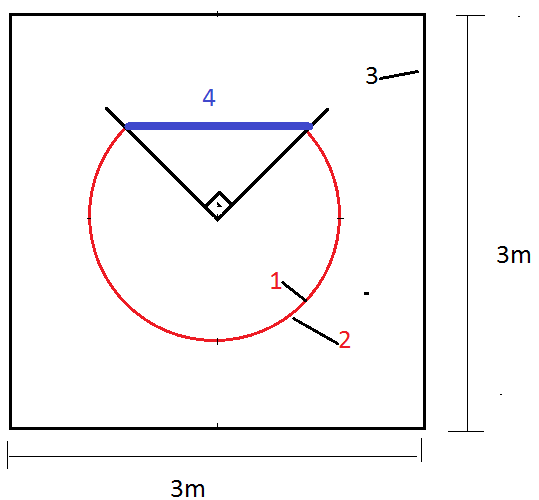
\includegraphics[scale=0.78]{./fig/1.png}
% \caption{\label{fig:1}1} 
% \end{center}
% \end{figure}

\myfig[scale=.78]{figPME2352-20111026-01}{}

1:
\[m_{1}\ddot{x}_{1}=k_{2}(x_{2}-x_{1})-k_{1}x_{1}\]
\[m_{2}\ddot{x}_{2}=-k_{2}(x_{2}-x_{1})-k_{3}x_{2}\]
2:
\[m_{1}\ddot{x}_{1}+(k_{1}+k_{2})x_{1}-k_{2}x_{2}=0\]
\[m_{2}\ddot{x}_{2}-k_{2}x_{1}+(k_{2}+k_{3})x_{2}=0\]
\\
Soluções:

\[x_{1}(t)=A_{1}\sin(\omega t + \phi)\]
\[x_{2}(t)=A_{2}\sin(\omega t + \phi)\]

\[x_{11}(t)=A_{11}\sin(\omega_{1} t + \phi _{1})\]
\[x_{21}(t)=\alpha A_{11}\sin(\omega_{1} t + \phi _{1})\]

\[x_{12}(t)=A_{12}\sin(\omega_{2} t + \phi _{2})\]
\[x_{22}(t)=\beta A_{12}\sin(\omega_{2} t + \phi _{2})\]
\\
Assim:
\[[-m_{1}\omega^{2}+(k_{1}+k_{2})A_{1}-k_{2}A_{2}]\sin(\omega t + \phi)=0\]
\[[-m_{2}\omega^{2}A_{2}-k_{2}A_{2}-(k_{2}+k_{3)}A_{2}]\sin(\omega t + \phi)=0\]

\[(k_{1}+k_{2}-m_{1}\omega^{2})A_{1}-k_{2}A_{2}=0\]
\[-k_{2}A_{1}+(k_{2}+k_{3}-m_{2}\omega^{2})A_{2}=0\]

\[\begin{pmatrix}
k_{1}+k_{2}-m_{1}\omega^{2} & -k_{2} \\ 
-k_{2} & k_{2}+k_{3}-m_{2}\omega_{2}
\end{pmatrix} \begin{pmatrix}
A_{1} \\ 
A_{2}
\end{pmatrix}=\begin{pmatrix}
0 \\ 
0
\end{pmatrix} \] 
\\

Soluiçao nao trivial:

\[\Delta=(k_{1}+k_{2}-m_{1}\omega_{2})(k_{2}+k_{3}-m_{1}\omega^{2})-k_{2}^{2}=0\]
\[m_{1}m_{2}\omega^{4}-[(k_{2}+k_{3})m_{1}+(k_{1}+k_{2})m_{2}]\omega^{2}+k_{1}k_{2}+k_{1}k_{3}+k_{2}k_{3}=0\]

\[\omega_{1,2}^{2}=\frac{(k_{2}+k_{3})m_{1}+(k_{1}+k_{2})m_{2}}{2m_{1}m_{2}}+- \sqrt{()^{2}- bla}\]

\[\omega_{1}^{2}>0\]
\[\omega_{2}^{2}>0\]
\\
Para $\omega^{2}=\omega_{1}^{2}$
\[(k_{1}+k_{2}-m_{1}\omega_{1}^{2})A_{11}-k_{2}A_{21}=0\]
\[A_{21}=\alpha A_{11}\]
\\
Para $\omega^{2}=\omega_{2}^{2}$
\[(k_{1}+k_{2}-m_{1}\omega_{2}^{2})A_{12}-k_{2}A_{22}=0\]
\[A_{21}=\beta A_{12}\]

\[
\begin{pmatrix}
2k-m\omega^{2} & -k \\ 
-k & 2k-m\omega_{2}
\end{pmatrix} \begin{pmatrix}
A_{1} \\ 
A_{2}
\end{pmatrix}=\begin{pmatrix}
0 \\ 
0
\end{pmatrix} 
\]
\\
Solução não-trivial

\[\Delta=(2k-m\omega^{2})-k^{2}=0\]
\[(2k-m\omega^{2})=+-k\]
\[\omega_{1}^{2}=\frac{k}{m}\]
\[\omega_{2}^{2}=\frac{3k}{m}\]
Para $\omega^{2}=\omega_{1}^{2}$

\[(2k-k)A_{11}-kA_{21}=0\]
Portanto $A_{21}=A_{11}$
\[-kA_{11}+(2k-k)A_{21}=0\]
\[x_{11}(t)=A_{11}\sin(\sqrt{\frac{k}{m}}t+\phi _{1})\]
\[x_{21}(t)=A_{11}\sin(\sqrt{\frac{k}{m}}t+\phi _{1})\]

Para $\omega^{2}=\omega_{2}^{2}$
\[(2k-3k)A_{12}-kA_{22}=0\]
Portanto $A_{22}=-A_{12}$
\[x_{12}(t)=A_{12}\sin(\sqrt{\frac{3k}{m}}t+\phi _{2})\]
\[x_{22}(t)=-A_{12}\sin(\sqrt{\frac{3k}{m}}t+\phi _{2})\]

% \begin{figure}[h]
% \begin{center}
% 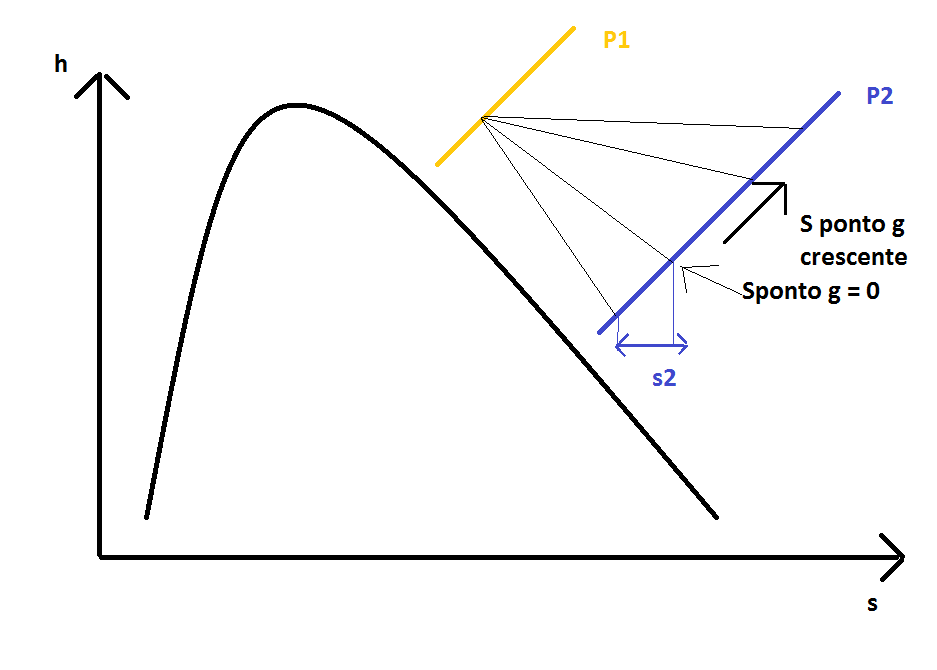
\includegraphics[scale=0.58]{./fig/2.png}
% \caption{\label{fig:2}2} 
% \end{center}
% \end{figure}

\myfig[scale=.58]{figPME2352-20111026-02}{}

Soluções:
\[x_{11}(t)=A_{11}\sin(\sqrt{\frac{k}{m}} t + \phi _{1})\]
\[x_{21}(t)= A_{11}\sin(\sqrt{\frac{k}{m}} t + \phi _{1})\]

\[x_{12}(t)=A_{12}\sin(\sqrt{\frac{3k}{m}} t + \phi _{2})\]
\[x_{22}(t)=- A_{12}\sin(\sqrt{\frac{3k}{m}} t + \phi _{2})\]
\[x_{1}(t)=x_{11}(t)+x_{12}(t)\]
\[x_{2}(t)=x_{21}(t)+x_{22}(t)\]

\[x_{1}(t)=A_{11}\sin(\omega_{1} t + \phi _{1})+A_{12}\sin(\omega_{2} t + \phi _{2})\]
\[x_{2}(t)=A_{11}\sin(\omega_{1} t + \phi _{1}) - A_{12}\sin(\omega_{2} t + \phi _{2})\]

\[x_{1}(t)=(A_{11}\cos(\phi _{1}))\sin(\omega _{1}t)+(A_{11}\sin(\phi _{1}))\cos(\omega _{1}t)+(A_{12}\cos(\phi _{2}))\sin(\omega _{2}t)+(A_{12}\sin(\phi _{2}))\cos(\omega _{2}t)\]
Onde:
\[(A_{11}\cos(\phi _{1}))=A\]
\[(A_{11}\sin(\phi _{1}))=B\]
\[(A_{12}\cos(\phi _{2}))=C\]
\[(A_{12}\sin(\phi _{2}))=D\]

Para $x_{2}(t)$, temos:
\[x_{2}(t)=A\sin(\omega _{1}t)+B\cos(\omega _{1}t)-C\sin(\omega _{2}t)-D\cos(\omega _{2}t)\]

Condições iniciais para t=0
\begin{itemize}
\item $x_{1}(0)=x_{10}$
\item $x_{2}(0)=x_{20}$
\item $\dot{x}_{1}(0)=\dot{x}_{10}$
\item $\dot{x}_{2}(0)=\dot{x}_{20}$
\end{itemize}

\[\dot{x}_{1}(t)=A\omega_{1}\cos(\omega_{1}t)-B\omega_{1}\sin(\omega_{1}t)+C\omega_{2}\cos(\omega_{2}t)-D\omega_{2}\sin(\omega_{2}t)\]

\[\dot{x}_{2}(t)=A\omega_{1}\cos(\omega_{1}t)-B\omega_{1}\sin(\omega_{1}t)-C\omega_{2}\cos(\omega_{2}t)+D\omega_{2}\sin(\omega_{2}t)\]

\[x_{10}=B+D\]
\[x_{20}=x_{2}(0)=B-D\]
\[\dot{x}_{1}(0)=\dot{x}_{10}=A\omega _{1}+C\omega _{2}\]
\[\dot{x}_{2}(0)=\dot{x}_{20}=A\omega _{1}-C\omega _{2}\]

\[B = \frac{x_{10}+x_{20}}{2}\]
\[D = \frac{x_{10}-x_{20}}{2}\]
\[A = \frac{\dot{x}_{10}+\dot{x}_{20}}{2\omega _{1}}\]
\[C = \frac{\dot{x}_{10}-\dot{x}_{20}}{2\omega _{2}}\]